
\noindent We've spent all of this energy on understanding the consequences of conformal symmetry on classical and quantum systems. Now, we finally take an example. The free massless boson provides a good building-block example, as it and copies of it can be used to construct all kinds of conformal field theories. \\

\noindent The Lagrangian of the (massless, $m=0$) free boson, from Klein-Gordon theory, where we have already solved the dynamics of this system, is

\begin{equation}
\mathcal{L} = \frac{1}{2} (\partial_\mu \phi)^2 - \frac{1}{2} m^2 \phi^2 = \frac{1}{2} (\partial_\mu \phi)^2.
\end{equation}

\noindent We set $m=0$ and drop the massive term, since $m \ne 0$ induces a length scale and the theory is then not conformally invariant. \\

\noindent Specialize to the Euclidean picture in $(2+0)$ dimensions, and write the action in complex coordinates

\begin{equation}
S = \frac{g}{2} \int dx \,\, (\partial_{x^0} - i \partial_{x^1} ) \phi (x) (\partial_{x^0} + i \partial_{x^1} ) \phi (x)
\end{equation}

\noindent Where $x = (x^0, x^1)$ and $dx = dx^0 dx^1$, and we write the action in terms of a differential operator (making four integrals)

\begin{equation}
S = \frac{1}{2} \int dx dy \,\, \phi (x) A (x,y) \phi (y)
\end{equation}

\noindent Where $A(x,y) = -g \delta (x-y) \partial_x^2$. \\

\noindent The Euclidean path integral prescription calculates $n$-point functions by the usual

\begin{equation}
\langle \hat{\phi}_1 \dots \hat{\phi}_n \rangle = \lim_{\beta \rightarrow \infty} \frac{\int \mathcal{D} \phi \,\, \phi_1 \dots \phi_n e^{-S}}{\int \mathcal{D} \phi \,\, e^{-S}}.
\end{equation}

\noindent Let's instead use the generating functional, as it is more convenient when working with a theory that is quadratic in the fields since we get all $n$-point correlations functions via differentation with respect to an external current field $J(x)$ and setting $J=0$. The generating functional is

\begin{equation}
Z[J] = Z[0] e^{\frac{1}{2} \int dx dy \,\, J(x) K(x,y) J(y)} \equiv \int \mathcal{D} \phi \,\, e^{-S + \int dx J(x) \phi (x)}
\end{equation}

\noindent Where $K(x,y)$ is the Green's function for a differential operator

\begin{equation}
-g \partial_x^2 K(x,y) = \delta (x-y).
\end{equation}

\noindent The solution to this Laplacian equation (by Fourier transform) is the same as the electrostatic potential of a point charge

\begin{equation}
K(x,y) = - \frac{1}{2\pi g} \log (\sqrt{(x-y)^2}).
\end{equation}

\noindent In polar coordinates

\begin{equation}
K(r) = -\frac{1}{2\pi g} \log (r) = -\frac{1}{4 \pi g} \log (r^2).
\end{equation}

\noindent Note that correlation nonintuitively \textit{grows} with separation. \\

\noindent The two-point correlation function is exactly the Green's function

\begin{equation}
\langle \hat{\phi} (x) \hat{\phi} (y) \rangle = \frac{\delta}{\delta J(x)} \frac{\delta}{\delta J(y)} Z[J] \Big{|}_{J=0} = K(x,y).
\end{equation}

\noindent Now, because we can, analytically continue the two-point function and define the complex coordinates

\begin{equation}
z = x^0 + i x^1 \text{ and } w = y^0 + i y^1
\end{equation}

\noindent And separate out the holomorphic and anti-holomorphic parts

\begin{equation}
\langle \hat{\phi} (z) \hat{\phi} (w) \rangle = - \frac{1}{4 \pi g} \log ((\bar{z} - \bar{w}) (z-w)) = -\frac{1}{4 \pi g} (\log (z-w) + \log (\bar{z} - \bar{w})).
\end{equation}

\noindent Recall that Wick's theorem will give all of the $n$-point functions in terms of the two-point functions, after some combinatorics, since we are working with a Gaussian theory, quadratic in the fields. \\

\noindent Now, with this form of the two-point functions, $\hat{\phi} (z)$ is \textit{not} a primary field, but $\partial_z \hat{\phi} (z)$ is a primary field. To check this, we will need to compute $\hat{T} (z)$ in terms of the stress-energy tensor. The holomorphic and anti-holomorphic two-point functions for the alleged primary fields are

\begin{align}
\langle \partial_z \hat{\phi} (z) \partial_w \hat{\phi} (w) \rangle &= - \frac{1}{4 \pi g} \frac{1}{(z-w)^2} \\
\langle \partial_{\bar{z}} \hat{\phi} (\bar{z}) \partial_{\bar{w}} \hat{\phi} (\bar{w}) \rangle &= - \frac{1}{4 \pi g} \frac{1}{(\bar{z}-\bar{w})^2}
\end{align}

\noindent Which has the correct form to transform as a primary field under a conformal transformation. So, the operator product expansion (OPE) of the two primary fields is 

\begin{equation}
\partial_z \hat{\phi} (z) \partial_w \hat{\phi} (w) \sim - \frac{1}{4 \pi g} \frac{1}{(z-w)^2}.
\end{equation}

\noindent Now, we will compute OPEs that include the stress-energy tensor. \\

\noindent \textbf{Intrepretations of the stress-energy tensor}: \\

\begin{enumerate}
\item Momentum flux of the $\mu^{\text{th}}$ component through the $\nu^{\text{th}}$ coordinate constant plane.
\item Conserved chrage corresponding to a translation in the $\mu^{\text{th}}$, or $\nu^{\text{th}}$, since symmetric, direction.
\item Variation of the action with respect to the metric $\frac{\delta S}{\delta g_{\mu\nu}}$.
\end{enumerate}

\noindent From Noether's theorem, for the Klein-Gordon field, the (traceless) stress-energy tensor is

\begin{equation}
T_{\mu\nu} = g ( \partial_\mu \phi \partial_\nu \phi - \frac{1}{2} \eta_{\mu\nu} \partial_\rho \phi \partial^\rho \phi ).
\end{equation}

\noindent Since this theory is quadratic in the fields, we quantize by ``putting hats on'' and applying normal-ordering

\begin{equation}
\hat{T}_{\mu\nu} = g \textbf{:} ( \partial_\mu \hat{\phi} \partial_\nu \hat{\phi} - \frac{1}{2} \eta_{\mu\nu} \partial_\rho \hat{\phi} \partial^\rho \hat{\phi} ) \textbf{:} .
\end{equation}

\noindent Apply the coordinate transformation to complex coordinates $(x^0, x^1) \rightarrow (z, \bar{z})$ (\textbf{Exercise})

\begin{align}
\hat{T} (z) = -2 \pi \hat{T}_{zz} &= 2\pi \frac{1}{4} \textbf{:} (\hat{T}_{00} - 2i \hat{T}_{10} - \hat{T}_{11}) \textbf{:} \\
&= -2\pi g \textbf{:} \partial_z \hat{\phi} (z)  \partial_z \hat{\phi} (z)  \textbf{:}.
\end{align}

\noindent Compute the OPE of the stress-energy tensor and the primary field, which is equivalent to ``putting $\hat{T} (z) \partial_w \hat{\phi} (w)$ inside an $n$-point function, computing its singular behavior as $z \rightarrow w$, and dropping the regular part''. Skipping several steps, by Wick's theorem and Taylor expansion about $w$

\begin{align}
\hat{T} (z) \partial_w \hat{\phi} (w) &= -2\pi g \left( \textbf{:} \wick{ \c {\partial_z \hat{\phi} (z)} \partial_z \hat{\phi} (z) \textbf{:} \c{ \partial_w \hat{\phi} (w) }} + \textbf{:} \partial_z \hat{\phi} (z) \wick{ \c {\partial_z \hat{\phi} (z)} \textbf{:} \c {\partial_w \hat{\phi} (w)}} \right) \\
&= -4\pi g \partial_z \hat{\phi} (z) \langle \partial_z \hat{\phi} (z) \partial_w \hat{\phi} (w) \rangle \\
&= \frac{1}{(z-w)^2} \partial_z \hat{\phi} (z) \\
&= \frac{1}{(z-w)^2} (\partial_w \hat{\phi} (w) + (z-w) \partial_w^2 \hat{\phi} (w) + \dots ) \\
&\sim \frac{1}{(z-w)^2} \partial_w \hat{\phi} (w) + \frac{1}{z-w} \partial_w^2 \hat{\phi} (w).
\end{align}

\noindent And we see that the OPE of $\hat{T} (z) \partial_w \hat{\phi} (w)$ is a primary field with $h=1$. \\

\noindent Now, compute the OPE of the stress-energy tensor with itself to see what the product of two local conformal transformations looks like, which we hope is another local conformal transformation. Again, by Wick's theorem and Taylor expansion

\begin{align}
\hat{T} (z) \hat{T} (w) &= 4 \pi^2 g^2 \textbf{:} \partial_z \hat{\phi} (z) \partial_z \hat{\phi} (z) \textbf{:} \,\, \textbf{:} \partial_w \hat{\phi} (w) \partial_w \hat{\phi} (w) \textbf{:} \\
&= \frac{1}{2} \frac{1}{(z-w)^4} - \frac{4\pi g}{(z-w)^2} \textbf{:} \partial_z \hat{\phi} (z) \partial_w \hat{\phi} (w) \textbf{:} \\
&\sim \frac{1}{2} \frac{1}{(z-w)^4} + \frac{2 \hat{T} (w)}{(z-w)^2} + \frac{\partial_w \hat{T} (w)}{z-w}.
\end{align}

\noindent And we see that the OPE of $\hat{T} (z) \hat{T} (w)$ is \textit{almost} a primary field with $h=2$, but it is spoiled bu the inverse quartic term. The quartic term arises, since the stress-energy tensor is of rank 2, and under dilations, behaves as $\hat{T} (z) \rightarrow \frac{1}{\lambda^2} \hat{T} (\lambda z)$. \\

\noindent In general, the OPE of the stress energy tensor with itself has the form

\begin{equation}
\hat{T} (z) \hat{T} (w) \sim \frac{c}{2} \frac{1}{(z-w)^4} + \frac{2 \hat{T} (w)}{(z-w)^2} + \frac{\partial_w \hat{T} (w)}{z-w}.
\end{equation}

\noindent We call $c$ the \textit{central charge}. It is the central extension of the Witt algebra, which comes from the fact that we allow $\text{Conf}(\mathbb{R}^{1,1})$ to act projectively. Since the two-point function is positive, the central charge is also positive $c \ge 0$. \\

\noindent Now, relate the OPE to an infinite Lie algebra that is obeyed by the generators of local conformal transformations: the \textit{Virasoro algebra}.

\subsection*{The Virasoro algebra}

\noindent Make a mode expansion (Laurent series defined in an annular region) of the stress-energy tensor

\begin{align}
\hat{T} (z) &\equiv \sum_{n \in \mathbb{Z}} z^{-n-2} \hat{L}_n \\
\hat{\bar{T}} (\bar{z}) &\equiv \sum_{n \in \mathbb{Z}} \bar{z}^{-n-2} \hat{\bar{L}}_n.
\end{align}

\noindent Invert these equations by multiplying by $z^{n+1}$, integrating around a circle, and applying the residue theorem

\begin{align}
\hat{L}_n &= \oint \frac{dz}{2\pi i} \,\, z^{n+1} \hat{T} (z) \\
\hat{\bar{L}}_n &= \oint \frac{d\bar{z}}{2\pi i} \,\, \bar{z}^{n+1} \hat{\bar{T}} (\bar{z}).
\end{align}

\noindent Our goal is to work out the Lie algebra that quantumly generates conformal symmetry. To do this, we employ a commutator and contour integral trick that we've used before. Consider

\begin{equation}
[ \hat{A}, \hat{B} ] = \oint_0 dw \oint_W dz \,\, \hat{a} (z) \hat{b} (w)
\end{equation}

\noindent Where $\hat{A} = \oint dz \, \hat{a} (z)$ and $\hat{B} = \oint dz \, \hat{b} (z)$. Consider the contours 

\begin{figure}[H]
	\centering
	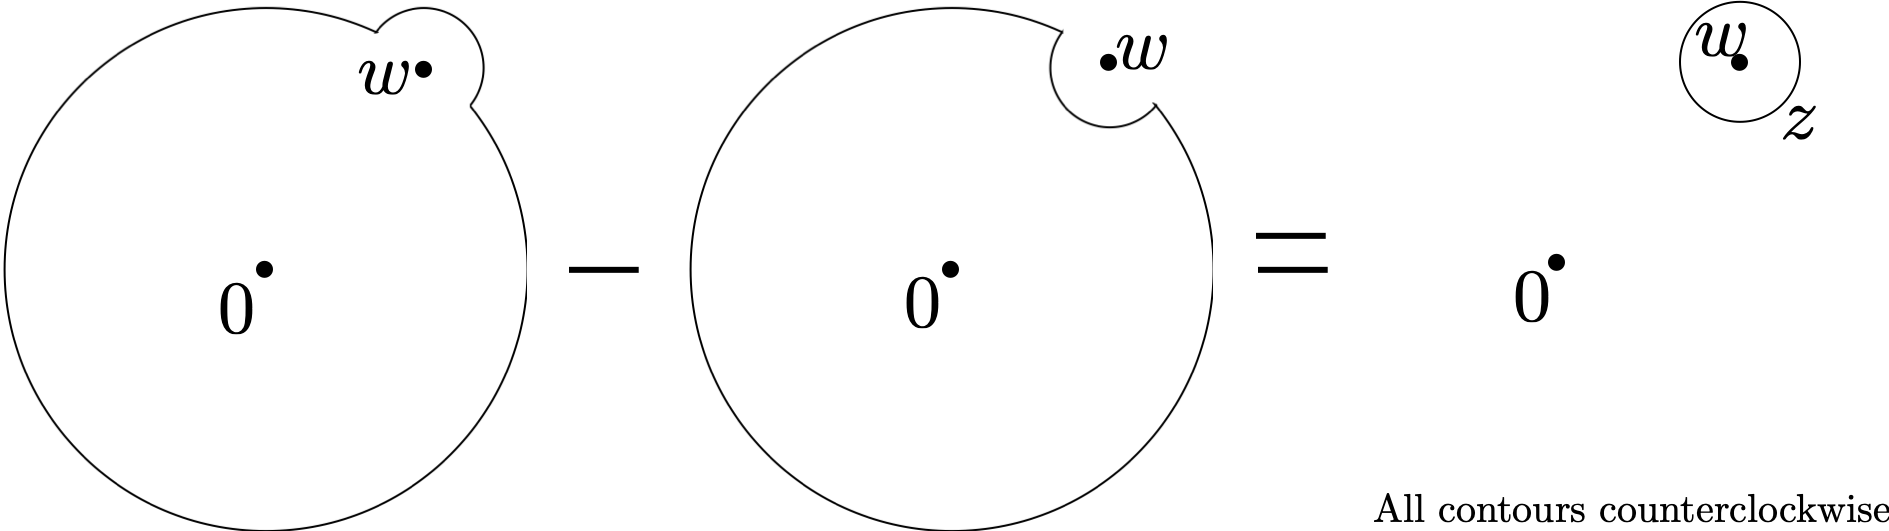
\includegraphics[width=4.5in]{images/contour_trick.png}
\end{figure}

\noindent Where we fix $w$ and then integrate around the circle around $w$ to obtain the difference between the larger contours. Use OPE to do the integral and pick up singular behavior as $z \rightarrow w$, and the regular behavior naturally goes to zero. \\

\noindent Use this calculate the commutator of the $\hat{L}_n$ operators

\begin{align}
[\hat{L}_n, \hat{L}_m ] &= \frac{1}{(2\pi i)^2} \oint_0 dw \, w^{m+1} \oint_W dz \, z^{n+1} \left( \frac{c}{2} \frac{1}{(z-w)^4} + \frac{2 \hat{T} (w)}{(z-w)^2} + \frac{\partial_w \hat{T} (w)}{z-w} + \text{regular} \right) \\
&= \frac{1}{2\pi i} \oint_0 dw \, w^{m+1} \left( \frac{c}{12} (n+1)n(n-1) w^{n-2} + 2(n+1) w^n \hat{T} (w) + w^{n+1} \partial_w \hat{T} (w) \right) \\
&= \frac{c}{12} n (n^2 - 1) \delta_{m+n,0} + 2 (n+1) \hat{L}_{m+n} - \frac{1}{2\pi i} \oint_0 dw \, (m+n+2) w^{m+n+1} \hat{T} (w) \\
[\hat{L}_n, \hat{L}_m ] &= \frac{c}{12} n (n^2 -1) \delta_{m+n,0} + (-m+n) \hat{L}_{m+n}.
\end{align}

\noindent And similarly for the anti-holomorphic part $\hat{\bar{L}}_n$. And the ``cross'' commutators are zero

\begin{equation}
[\hat{L}_n, \hat{\bar{L}}_m ] = 0.
\end{equation}

\noindent The delta function piece of the commutator relation is a phase factor of the central extension of the Lie algebra, due to representing the Lie algebra projectively. This is the algebra of local conformal transformations, and is an infinite-dimensional Lie algebra. It contains the closed subalgebra formed by $\{ \hat{L}_{-1}, \hat{L}_0, \hat{L}_1 \}$, which is isomorphic to the $SL_2 (\mathbb{C})$ algebra. The global conformal transformations correspond to this three dimensional, or rank 1, subalgebra.
